\section{Categories of Urban Heat Island}
	
	There are two types of urban heat island based on how they are formed and how high they reach:
	surface urban heat islands and atmospheric urban heat islands (Figure \ref{fig:urban-heat-types}).
	
	\begin{figure}
		\centering
		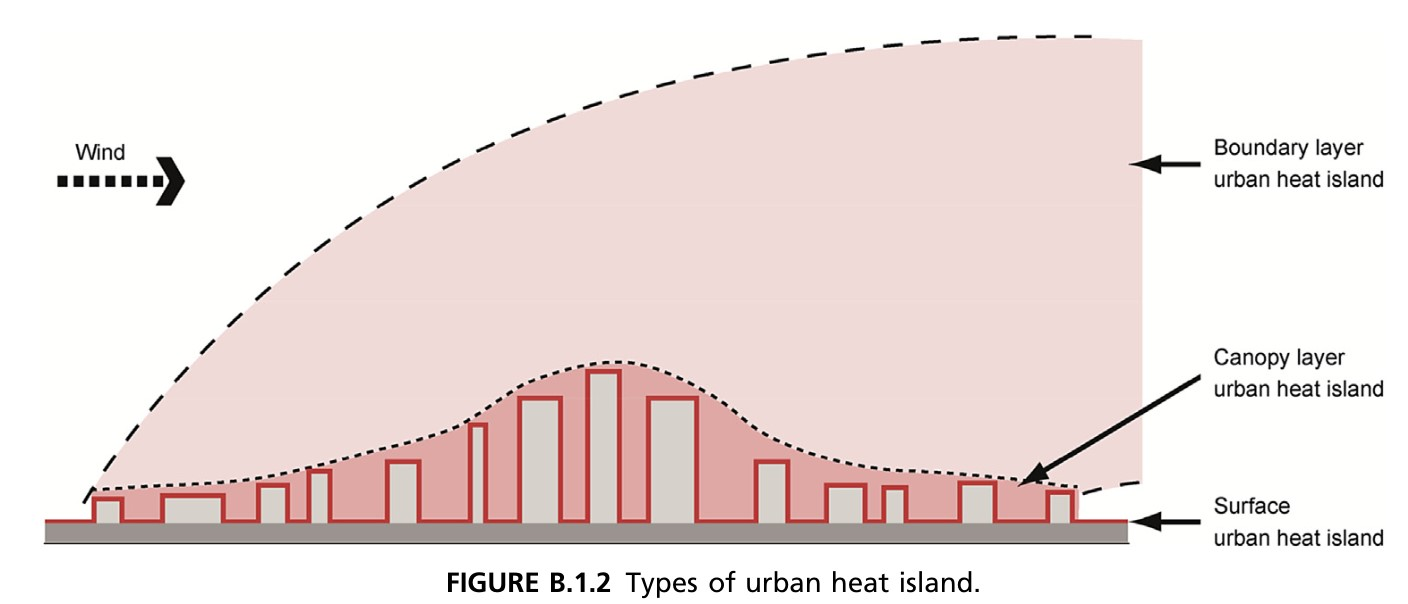
\includegraphics[width=\textwidth]{urban-heat-types}
		\caption{Types of urban heat island. Taken from \textcite{Khan2021}.}
		\label{fig:urban-heat-types}
	\end{figure}
	
	Surface urban heat islands refer to the warmer surface of urbanized areas compared to the temperature of rural surfaces, and is primarily measured by satellite thermal remote sensing data (\cite{Zhou2018}). 
	How hot a surface can reach depends on its properties.
	Dry and exposed surfaces such as roofs and pavements can become significantly hotter than the air, while shaded and moist surfaces remain as hot as the air (\cite{Khan2021}). 
	
	Atmospheric urban heat islands refer to the warmer air temperature of urbanized areas compared to the air temperature of rural areas.
	This category of urban heat island is subdivided into two more classifications:
	the canopy layer and the boundary layer (\cite{Zhou2018}).
	The canopy layer starts from the ground up to the treetops and rooftops, 
	while the boundary starts from the treetops and rooftops and extends up until point where the urban area does not affect the atmosphere (\cite{Khan2021}).
	Canopy temperatures are typically measured by sensors from meteorological stations or vehicles,
	while boundary temperatures are measured by sensors from specialized platforms such as tall towers or aircrafts (\cite{Zhou2018}).

\section{Radiant Heat and Energy Balance}
	The heating of the Earth is caused by the exchange of energy between the Sun, the Earth's atmosphere, and the Earth's surface.
	The solar rays incident on the Earth, combined with the Earth's rotation, creates a diurnal energy balance.
	These energy exchanges can be associated with an energy flux density, with units $\si{W.m^{-2}}$.
	
	\begin{figure}	
		\centering
		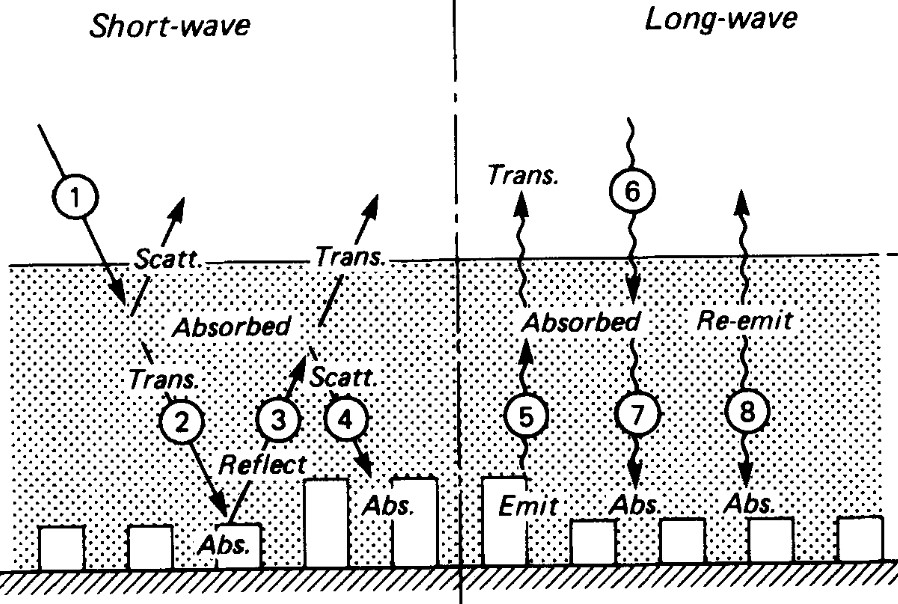
\includegraphics{radiation-budget}
		\caption{Radiation budget.}
		\label{fig:radiation-budget}
	\end{figure}

	Figure \ref{fig:radiation-budget} depicts a schematic of the fluxes present in the heating of the Earth.
	Shortwave radiation from the sun enters the urban boundary layer.
	Some of the radiation reach the surface with flux magnitude $Q_{S\downarrow}$.
	The other radiation is reflected or scattered back upward with flux magnitude $Q_{S\uparrow}$.
	The atmosphere emits longwave radiation, with some
	reaching the Earth’s surface with flux magnitude $Q_{L\downarrow}$.
	The Earth’s surface also emits longwave radiation upward with flux magnitude $Q_{L\uparrow}$. 
	The net radiation flux $Q^*$ then is given by
	\begin{equation}
		Q^* = Q_{S\downarrow} - Q_{S\uparrow} + Q_{L\downarrow} - Q_{L\uparrow}.
	\end{equation}
		
	In a rural environment, the surplus of energy provided by $Q^*$ is shared by the soil and the air.
	Heat is dissipated via conduction to the soil with flux $Q_G$,
		and via convection of sensible and latent heat with fluxes $Q_H$ and $Q_E$ respectively. 
	Thus,
	\begin{equation}
		Q^* = Q_G + Q_H + Q_E.
	\end{equation}
	An urban environment, however, modifies the energy balance in multiple ways:
	\begin{enumerate}
		\item \textbf{Canyon geometry of buildings.}
		Dense tall buildings create a canyon geometry,
			which causes radiation to get trapped in between the vertical surfaces through multiple reflections.
		This gives a greater absorption of shortwave radiation.
		This also causes a reduction of wind speed, which trap warm air.
		
		\item \textbf{Construction materials.}
		Buildings and paved surfaces are made with materials that have great heat absorption and heat storage.
		
		\item \textbf{Removal of plants and soil.}
		The replacement of plants and moist soil with paved and waterproof surfaces reduces evapotranspiration.
		More of the net radiation flux is thus converted into sensible heat, rather than latent heat.
		
		\item \textbf{Air pollution.}
		A polluted atmosphere has greater absorption and re-emission of radiation, thus increasing longwave radiation flux.
		
		\item \textbf{Anthropogenic heat.}
		There is a release of heat from man-made activities such as from
			the combustion of fuels in vehicles,
			industrial processes, and
			air-conditioning in rooms.
		Humans also release heat and moisture from metabolism, but is not as significant compared to the activities mentioned.
	\end{enumerate}

	Accordingly, extra terms are needed in the energy balance equation in order to account for these factors in the urban environment.
	The energy balance equation thus becomes
	\begin{equation}
		Q^* + Q_F= Q_H + Q_E + \Delta Q_S + \Delta Q_A,
	\end{equation}
	where $Q_F$ is the anthropogenic heat release flux,
	$\Delta Q_S$ is the storage heat flux,
	$\Delta Q_A$ is the net advection that lets heat go through the sides of the volume, and
	other terms as defined as before.
%\section{Radiative Transfer}
%
%	The sun heats up the atmosphere and surface of Earth through radiative transfer, the transfer of energy via electromagnetic radiation.
%	When radiation interacts with matter, it may either be absorbed, emitted, reflected, scattered, or simply transmitted.
%	The outcome depends on the wavelength of the radiation as well as the properties of the material interacting with the radiation.
%
%	\subsection{Reflection, Scattering, and Albedo}
%	%
%	%As solar radiation travels through the atmosphere,
%	%\blindtext
%	Energy may be returned to space through reflection or scattering.
%	
%	Albedo is defined as the ``ratio of the amount of solar radiation reflected by a surface to the amount received by it'' (\cite{Stewart2012}).
%	
%
%	\subsection{Absorption and Emission}
%	
%	\blindtext
%
%\section{Urban Heat Island}
%
%
%
%	\subsection{Factors Causing Urban Heat Islands}
%	
%	Different climatic and nonclimatic factors are responsible for causing urban heat islands.
%	\citeauthor{Bridgman1995} (\citeyear{Bridgman1995}, as cited in \cite{Khan2021}) lists five major ways in which urbanization can influence a city's climate:
%	\begin{itemize}
%		\item by replacing natural surfaces with asphalts, concrete, and glasses;
%		\item by replacing natural shape with blocky, angular, towering structures;
%		\item by releasing anthropogenic heat into the urban atmosphere;
%		\item by routing flow of surface runoff and preventing infiltration; and
%		\item by emitting pollutants into the urban atmosphere.
%	\end{itemize}